% Báo cáo dự án LexProof. Biên dịch: lualatex bao-cao-du-an.tex (hai lần, để có mục lục).
% Hình HLD và LLD dựng riêng trước (cũng dùng cho slide):
%   lualatex -jobname=fig-hld "\def\fig{fig-hld}% Biên dịch riêng một hình (cho slide): lualatex "\def\fig{fig-hld}% Biên dịch riêng một hình (cho slide): lualatex "\def\fig{fig-hld}% Biên dịch riêng một hình (cho slide): lualatex "\def\fig{fig-hld}\input{fig-standalone}"
\documentclass[border=6pt]{standalone}
\usepackage{fontspec}
\directlua{luaotfload.add_fallback("symfb",{"SegoeUISymbol:mode=harf;","CambriaMath:mode=harf;"})}
\setmainfont{Times New Roman}[RawFeature={fallback=symfb}]
\setsansfont{Arial}[RawFeature={fallback=symfb}]
\setmonofont{Cascadia Mono}[Scale=0.78,RawFeature={fallback=symfb}]
\usepackage{xcolor}
\definecolor{accentc}{HTML}{1F4E79}
\definecolor{warnc}{HTML}{8A3B12}
\usepackage{tikz}
\usetikzlibrary{positioning,arrows.meta,fit,backgrounds,shapes.geometric,calc}
\begin{document}
\input{\fig}
\end{document}
"
\documentclass[border=6pt]{standalone}
\usepackage{fontspec}
\directlua{luaotfload.add_fallback("symfb",{"SegoeUISymbol:mode=harf;","CambriaMath:mode=harf;"})}
\setmainfont{Times New Roman}[RawFeature={fallback=symfb}]
\setsansfont{Arial}[RawFeature={fallback=symfb}]
\setmonofont{Cascadia Mono}[Scale=0.78,RawFeature={fallback=symfb}]
\usepackage{xcolor}
\definecolor{accentc}{HTML}{1F4E79}
\definecolor{warnc}{HTML}{8A3B12}
\usepackage{tikz}
\usetikzlibrary{positioning,arrows.meta,fit,backgrounds,shapes.geometric,calc}
\begin{document}
\input{\fig}
\end{document}
"
\documentclass[border=6pt]{standalone}
\usepackage{fontspec}
\directlua{luaotfload.add_fallback("symfb",{"SegoeUISymbol:mode=harf;","CambriaMath:mode=harf;"})}
\setmainfont{Times New Roman}[RawFeature={fallback=symfb}]
\setsansfont{Arial}[RawFeature={fallback=symfb}]
\setmonofont{Cascadia Mono}[Scale=0.78,RawFeature={fallback=symfb}]
\usepackage{xcolor}
\definecolor{accentc}{HTML}{1F4E79}
\definecolor{warnc}{HTML}{8A3B12}
\usepackage{tikz}
\usetikzlibrary{positioning,arrows.meta,fit,backgrounds,shapes.geometric,calc}
\begin{document}
\input{\fig}
\end{document}
"
%   lualatex -jobname=fig-lld "\def\fig{fig-lld}% Biên dịch riêng một hình (cho slide): lualatex "\def\fig{fig-hld}% Biên dịch riêng một hình (cho slide): lualatex "\def\fig{fig-hld}% Biên dịch riêng một hình (cho slide): lualatex "\def\fig{fig-hld}\input{fig-standalone}"
\documentclass[border=6pt]{standalone}
\usepackage{fontspec}
\directlua{luaotfload.add_fallback("symfb",{"SegoeUISymbol:mode=harf;","CambriaMath:mode=harf;"})}
\setmainfont{Times New Roman}[RawFeature={fallback=symfb}]
\setsansfont{Arial}[RawFeature={fallback=symfb}]
\setmonofont{Cascadia Mono}[Scale=0.78,RawFeature={fallback=symfb}]
\usepackage{xcolor}
\definecolor{accentc}{HTML}{1F4E79}
\definecolor{warnc}{HTML}{8A3B12}
\usepackage{tikz}
\usetikzlibrary{positioning,arrows.meta,fit,backgrounds,shapes.geometric,calc}
\begin{document}
\input{\fig}
\end{document}
"
\documentclass[border=6pt]{standalone}
\usepackage{fontspec}
\directlua{luaotfload.add_fallback("symfb",{"SegoeUISymbol:mode=harf;","CambriaMath:mode=harf;"})}
\setmainfont{Times New Roman}[RawFeature={fallback=symfb}]
\setsansfont{Arial}[RawFeature={fallback=symfb}]
\setmonofont{Cascadia Mono}[Scale=0.78,RawFeature={fallback=symfb}]
\usepackage{xcolor}
\definecolor{accentc}{HTML}{1F4E79}
\definecolor{warnc}{HTML}{8A3B12}
\usepackage{tikz}
\usetikzlibrary{positioning,arrows.meta,fit,backgrounds,shapes.geometric,calc}
\begin{document}
\input{\fig}
\end{document}
"
\documentclass[border=6pt]{standalone}
\usepackage{fontspec}
\directlua{luaotfload.add_fallback("symfb",{"SegoeUISymbol:mode=harf;","CambriaMath:mode=harf;"})}
\setmainfont{Times New Roman}[RawFeature={fallback=symfb}]
\setsansfont{Arial}[RawFeature={fallback=symfb}]
\setmonofont{Cascadia Mono}[Scale=0.78,RawFeature={fallback=symfb}]
\usepackage{xcolor}
\definecolor{accentc}{HTML}{1F4E79}
\definecolor{warnc}{HTML}{8A3B12}
\usepackage{tikz}
\usetikzlibrary{positioning,arrows.meta,fit,backgrounds,shapes.geometric,calc}
\begin{document}
\input{\fig}
\end{document}
"
\documentclass[12pt,a4paper]{article}

\usepackage{fontspec}
\directlua{luaotfload.add_fallback("symfb",{"SegoeUISymbol:mode=harf;","CambriaMath:mode=harf;"})}
\setmainfont{Times New Roman}[RawFeature={fallback=symfb}]
\setsansfont{Arial}[RawFeature={fallback=symfb}]
\setmonofont{Cascadia Mono}[Scale=0.78,RawFeature={fallback=symfb}]

\usepackage[a4paper,left=2.8cm,right=2.3cm,top=2.4cm,bottom=2.4cm]{geometry}
\usepackage{setspace}\setstretch{1.08}
\usepackage{microtype}
\usepackage{xcolor}
\definecolor{accent}{HTML}{1F4E79}
\definecolor{soft}{HTML}{EEF3F8}
\definecolor{warn}{HTML}{8A3B12}
\colorlet{accentc}{accent}
\colorlet{warnc}{warn}
\usepackage{titlesec}
\titleformat{\section}{\Large\bfseries\color{accent}}{\thesection.}{0.6em}{}
\titleformat{\subsection}{\large\bfseries\color{accent}}{\thesubsection}{0.6em}{}
\titleformat{\subsubsection}{\normalsize\bfseries}{\thesubsubsection}{0.6em}{}
\titlespacing*{\section}{0pt}{1.4em}{0.6em}
\titlespacing*{\subsection}{0pt}{1.0em}{0.4em}
\usepackage{booktabs,tabularx,array,longtable}
\renewcommand{\arraystretch}{1.25}
\newcolumntype{L}{>{\raggedright\arraybackslash}X}
\usepackage{enumitem}\setlist{itemsep=2pt,topsep=4pt}
\usepackage{float}
\usepackage{caption}\captionsetup{font=small,labelfont={bf,color=accent},labelsep=period}
\captionsetup[figure]{name=Hình}
\captionsetup[table]{name=Bảng}
\usepackage{fancyvrb}
\fvset{fontsize=\small,frame=single,framesep=6pt,rulecolor=\color{accent!50},xleftmargin=4pt,xrightmargin=4pt}
\usepackage{tikz}
\usetikzlibrary{positioning,arrows.meta,fit,backgrounds,shapes.geometric,calc}
\usepackage{tcolorbox}
\newtcolorbox{keybox}[1][]{colback=soft,colframe=accent,boxrule=0.6pt,arc=2pt,left=8pt,right=8pt,top=6pt,bottom=6pt,#1}
\newtcolorbox{warnbox}[1][]{colback=warn!5,colframe=warn,boxrule=0.6pt,arc=2pt,left=8pt,right=8pt,top=6pt,bottom=6pt,#1}
\usepackage{fancyhdr}
\pagestyle{fancy}\fancyhf{}
\fancyhead[L]{\small\color{accent}LexProof: kiểm tra tính nhất quán của văn bản luật bằng Lean 4}
\fancyhead[R]{\small\thepage}
\renewcommand{\headrulewidth}{0.4pt}
\usepackage[hidelinks]{hyperref}
\renewcommand{\contentsname}{Mục lục}
\renewcommand{\refname}{Tài liệu tham khảo}

\newcommand{\code}[1]{\texttt{#1}}
\newcommand{\term}[1]{\textbf{#1}}

\begin{document}

% ---------------------------------------------------------------- Trang bìa
\begin{titlepage}
\centering
\vspace*{1.2cm}
{\large BÁO CÁO DỰ ÁN\par}
\vspace{1.6cm}
{\fontsize{30}{36}\selectfont\bfseries\color{accent} LexProof\par}
\vspace{0.6cm}
{\Large Kiểm tra tính nhất quán logic của văn bản luật tiếng Việt\\ bằng chứng minh hình thức trong Lean 4\par}
\vspace{1.4cm}
\begin{tcolorbox}[colback=soft,colframe=accent,boxrule=0.6pt,arc=2pt,width=0.86\textwidth]
\small Hệ thống nhận một văn bản luật, chuyển từng điều khoản thành dữ liệu có cấu trúc nhờ AI và người duyệt, rồi dùng
\emph{kernel} của trợ lý chứng minh Lean 4 để chứng minh rằng phần đã mã hóa không có hai quy định trái nhau, hoặc chỉ ra
tình huống cụ thể mà chúng trái nhau. Văn bản thử nghiệm: Luật Phòng, chống tác hại của rượu, bia số 44/2019/QH14.
\end{tcolorbox}
\vfill
\begin{tabular}{rl}
Sinh viên thực hiện: & Nguyễn Việt Phương\\
Người duyệt bản mã hóa: & Vũ Đức Phong\\
Giảng viên hướng dẫn: & Nguyễn Phương Thái\\
Học phần: & [Tên học phần dự án]\\
\end{tabular}
\vspace{1.2cm}

{\large Tháng 11 năm 2026\par}
\end{titlepage}

\tableofcontents
\clearpage

% ================================================================ 1
\section{Giới thiệu và phát biểu bài toán}

\subsection{Bối cảnh}

Một văn bản luật là một tập hợp các quy định: điều này \emph{cấm} một hành vi, điều kia \emph{bắt buộc} một hành vi khác,
điều khác nữa \emph{cho phép} một việc trong những điều kiện nhất định. Văn bản dài hàng chục điều, được soạn bởi nhiều người
và sửa qua nhiều vòng, nên có thể chứa những chỗ \term{mâu thuẫn}: trong cùng một tình huống, một điều khoản bắt làm
còn một điều khoản khác cấm làm, mà văn bản không nói bên nào được ưu tiên. Người tuân thủ luật khi đó không thể làm đúng cả
hai.

Ví dụ minh họa (giả định, không lấy từ luật thật):
\begin{itemize}
  \item Điều A: \emph{Cấm bán rượu, bia cho người chưa đủ 18 tuổi.}
  \item Điều B: \emph{Cơ sở có giấy phép được bán rượu, bia cho khách hàng.}
\end{itemize}
Một cửa hàng có giấy phép bán rượu cho một khách 17 tuổi: Điều B cho phép, Điều A cấm. Nếu văn bản không nói Điều A là ngoại
lệ của Điều B, thì đó là một \term{xung đột chuẩn tắc} (normative conflict). Ở ví dụ này người đọc nhận ra ngay. Với một văn
bản 36 điều, hàng trăm điều kiện đan xen và các ngoại lệ lồng nhau («trừ trường hợp quy định tại khoản 3 Điều này»), việc rà
soát bằng tay vừa tốn công vừa dễ sót.

\subsection{Phát biểu bài toán}

\begin{keybox}
\textbf{Đề bài.} Xây dựng \textbf{LexProof}: một hệ thống giúp người đọc luật tìm ra những quy định mâu thuẫn nhau trong
\emph{một} văn bản luật tiếng Việt. Khi tìm thấy, hệ thống chỉ ra tình huống cụ thể gây mâu thuẫn. Khi không tìm thấy, hệ
thống đưa ra một \textbf{chứng minh toán học được máy kiểm lại}, chứ không chỉ một câu trả lời của chương trình.
\end{keybox}

\paragraph{Sản phẩm gồm những gì.}
\begin{enumerate}
  \item \textbf{Một thư viện Lean 4} là lõi của hệ thống: định nghĩa chính xác thế nào là quy định và thế nào là xung đột,
    bộ kiểm xung đột, các định lý chứng minh bộ kiểm đúng, và mỗi điều luật đã duyệt là một module trong thư viện.
  \item \textbf{Một bộ công cụ Python} quanh lõi: tách văn bản, sinh và đọc phiếu duyệt, đưa bản dịch đã duyệt vào thư viện
    Lean, sinh bản kết quả kiểm tra.
  \item \textbf{Một quy trình duyệt có truy vết}: mỗi bản dịch phải được người duyệt từng dòng trên phiếu, phiếu ghi mã băm
    của đúng tệp được duyệt.
  \item \textbf{Bản kết quả kiểm tra}: tệp tiếng Việt do hệ thống tự sinh sau mỗi lần kiểm (ví dụ \code{reports/law44-2026-11-25.md}), nêu kết luận, phạm vi đã mã hóa, các định lý làm căn cứ, phản ví dụ nếu có, và những gì không được chứng minh. Đây là thứ người dùng nhận được; nó khác với báo cáo dự án này.
\end{enumerate}

\paragraph{Văn bản luật được biến đổi bằng gì.} Hệ thống không đọc thẳng chữ luật để kết luận. Chữ luật đi qua một chuỗi
biến đổi; mỗi bước có công cụ riêng và có nơi chịu trách nhiệm về độ đúng của bước đó (Bảng~\ref{tab:transform}).

\begin{table}[H]
\centering\small
\caption{Chuỗi biến đổi từ chữ luật tới kết luận.}
\label{tab:transform}
\begin{tabularx}{\textwidth}{>{\raggedright\arraybackslash}p{4.4cm}>{\raggedright\arraybackslash}p{4.3cm}L}
\toprule
Biến đổi & Công cụ & Ai bảo đảm bước này đúng\\
\midrule
Văn bản thành các điều, khoản, điểm có mã tham chiếu & Bộ tách văn bản (Python) & Lean kiểm mọi mã tham chiếu đều phân tích được\\
Mỗi điều thành các \emph{norm}: dữ liệu có cấu trúc gồm tính chất, hành vi, điều kiện, ngoại lệ, nguồn & Mô hình ngôn ngữ lớn
(Claude), theo bảng thuật ngữ chung & Không ai: bước này không được tin. Công cụ kiểm trích dẫn nguyên văn và tên gọi\\
Norm đề xuất thành norm đã duyệt & Phiếu duyệt & \textbf{Người duyệt}: chịu trách nhiệm bản mã hóa đúng nghĩa chữ luật\\
Norm đã duyệt thành module Lean & Công cụ \emph{promote} (Python) & Build Lean phải đạt, nếu không thì hoàn tác\\
Module Lean thành kết luận & Bộ kiểm trong Lean, chạy bởi kernel (\code{decide +kernel}) & \textbf{Kernel Lean 4}: kết luận là
một định lý đã được kiểm\\
Kết luận thành bản kết quả kiểm tra & Hàm in của Lean (\code{analyzeReport}) và \code{report.py} & Bản kết quả chép lại đầu ra của
Lean, không ai sửa tay\\
\bottomrule
\end{tabularx}
\end{table}

\paragraph{Chiều dữ liệu.} Dữ liệu nạp vào là chữ của văn bản luật (lấy từ Công báo); dữ liệu nhận ra là bản kết quả kiểm tra. Bản kết quả
cáo nêu đúng một trong ba kết luận, luôn kèm phạm vi đã mã hóa và trạng thái duyệt:
\begin{enumerate}[label=(\arabic*)]
  \item \textbf{Tìm thấy xung đột}: cặp điều khoản và một tình huống cụ thể mà ở đó chúng trái nhau;
  \item \textbf{Nhất quán trên phần đã mã hóa}: có chứng minh rằng không tồn tại tình huống nào như vậy, \emph{trong phần
    văn bản đã được mã hóa và duyệt};
  \item \textbf{Không biết}: dữ liệu không hợp lệ hoặc không đủ để kết luận (hệ thống từ chối thay vì đoán).
\end{enumerate}

Hai quy định được coi là \term{xung đột} khi đồng thời thỏa bốn điều kiện: (i) cùng điều chỉnh một hành vi; (ii) có tính
chất trái nhau (cấm với bắt buộc, hoặc cấm với cho phép); (iii) cùng áp dụng trong ít nhất một tình huống, tức là điều kiện
của cả hai đều đúng và không ngoại lệ nào loại chúng; (iv) văn bản không nói rõ bên nào được ưu tiên.

Ngoài xung đột, hệ thống còn kiểm \term{tham chiếu treo} (một điều dẫn chiếu tới khoản không tồn tại) và, ở mức ưu tiên
thấp hơn, ba \term{dấu hiệu lỗi soạn thảo}: quy định không bao giờ áp dụng được (\emph{chết}), quy định bị một quy định khác
bao trùm hoàn toàn (\emph{thừa}), và ngoại lệ không bao giờ có tác dụng.

\subsection{Phạm vi}

Dự án chỉ làm \term{Level 1}: tính nhất quán \emph{bên trong một văn bản}. Mâu thuẫn \emph{giữa các văn bản} (luật với
nghị định, văn bản cũ với văn bản mới, thứ bậc hiệu lực) là Level 2, để làm sau; dữ liệu vẫn giữ sẵn các trường mã văn bản,
loại văn bản và ngày hiệu lực để mở rộng.

Hệ thống \textbf{không} là công cụ tư vấn pháp lý: nó không nói một hành vi cụ thể là hợp pháp hay trái luật, và không bao
giờ kết luận «văn bản đúng». Những khái niệm mở của luật như «hợp lý», «nghiêm trọng», «dành cho người chưa đủ 18 tuổi» được
giữ là \term{tham số}: hệ thống xét mọi giá trị có thể của chúng chứ không tự quyết giá trị.

\subsection{Hai loại «đúng» cần tách bạch}

Đây là ý quan trọng nhất của dự án.
\begin{itemize}
  \item \term{Đúng hình thức (soundness)}: nếu hệ thống nói «nhất quán», thì điều đó đúng \emph{về mặt toán học} với bản mã
    hóa. Lean 4 bảo đảm phần này: mỗi kết luận là một định lý được kernel kiểm, không thể «tin nhầm» một chương trình có lỗi.
  \item \term{Trung thực với luật (faithfulness)}: bản mã hóa có đúng nghĩa của chữ luật không. Không chương trình nào chứng
    minh được điều này; nó chỉ được kiểm bằng con người đọc và đối chiếu.
\end{itemize}
Một chứng minh hoàn hảo trên một bản mã hóa sai thì vô giá trị. Vì vậy hệ thống dùng AI để \emph{soạn} bản mã hóa nhưng
bắt buộc mọi dòng phải qua \emph{người duyệt}, và mọi bản kết quả kiểm tra đều ghi rõ cái gì được chứng minh, cái gì chỉ được tin.

\subsection{Đóng góp}

\begin{enumerate}
  \item Một lõi kiểm xung đột viết trong Lean 4 với các định lý liên kết: kết quả «nhất quán» \emph{được chứng minh} là không
    có xung đột ở bất kỳ tình huống nào; kết quả «xung đột» \emph{được chứng minh} là có tình huống thật.
  \item Một quy trình đưa văn bản vào hệ thống có kiểm soát: AI dịch, người duyệt trên phiếu, mọi phiếu ghim mã băm sha256
    của đúng tệp được duyệt, và công cụ từ chối mọi thứ chưa duyệt.
  \item Kiểm xung đột \emph{giữa các hành vi khác tên} qua «cạnh kéo theo» có chứng minh ngữ nghĩa, kèm cách duyệt theo nhu
    cầu: người duyệt chỉ phải xem những cạnh thật sự dẫn tới xung đột.
  \item Kiểm dấu hiệu lỗi soạn thảo bằng \emph{chứng nhân}: một công cụ không tin cậy tìm ví dụ, kernel kiểm ví dụ.
\end{enumerate}

% ================================================================ 2
\section{Cơ sở lý thuyết}

\subsection{Logic chuẩn tắc: cấm, bắt buộc, cho phép}

Logic chuẩn tắc (deontic logic) nghiên cứu các khái niệm «phải», «không được», «được phép». Mỗi quy định trong hệ thống được
biểu diễn thành một \term{norm} gồm: một \emph{tính chất} (modality: bắt buộc, cấm, cho phép), một \emph{hành vi} bị điều
chỉnh, một \emph{điều kiện} áp dụng, danh sách \emph{ngoại lệ}, thông tin \emph{ưu tiên}, và \emph{nguồn} (điều, khoản,
điểm của luật). Hai tính chất được coi là trái nhau theo Bảng~\ref{tab:incompat}.

\begin{table}[H]
\centering
\caption{Quan hệ trái nhau giữa các tính chất (đối xứng; một tính chất không trái với chính nó).}
\label{tab:incompat}
\begin{tabular}{lccc}
\toprule
 & bắt buộc & cấm & cho phép\\
\midrule
bắt buộc & --- & \textbf{trái} & ---\\
cấm & \textbf{trái} & --- & \textbf{trái}\\
cho phép & --- & \textbf{trái} & ---\\
\bottomrule
\end{tabular}
\end{table}

Bắt buộc và cho phép không trái nhau (được phép làm điều mình phải làm). Định nghĩa xung đột theo lý thuyết pháp luật
(Kelsen; Vranes) rộng hơn: \emph{hai norm xung đột khi tuân thủ norm này kéo theo vi phạm norm kia}. Định nghĩa rộng này bao
cả trường hợp hai hành vi khác tên nhưng hành vi này kéo theo hành vi kia (ví dụ «thu hồi hàng» kéo theo «vận chuyển hàng»);
mục~\ref{sec:entail} trình bày cách hệ thống xử lý trường hợp đó.

Luật thường tự giải quyết xung đột bằng nguyên tắc ưu tiên: quy định riêng thắng quy định chung (\emph{lex specialis}), quy
định sau thắng quy định trước (\emph{lex posterior}), văn bản cao thắng văn bản thấp (\emph{lex superior}). Trong Level 1, hệ
thống chỉ dùng ưu tiên khi bản mã hóa ghi rõ «norm này thắng norm kia»; một cặp mà cả hai bên cùng tự nhận thắng là một
\emph{chu trình ưu tiên} và bị báo lỗi.

\subsection{Mô hình tình huống hữu hạn}

Để máy kiểm được «có tồn tại tình huống nào mà hai norm cùng áp dụng không», mỗi tình huống được mô tả bằng một số hữu hạn
\term{atom}: biến đúng/sai (ví dụ \code{dia\_diem\_co\_so\_y\_te}: địa điểm là cơ sở y tế) hoặc biến có vài giá trị
(ví dụ \code{do\_con}: «dưới 15 độ» / «từ 15 độ trở lên»). Mỗi atom và mỗi giá trị đều ghi khoản luật làm nguồn. Điều kiện
của norm là một biểu thức logic (và, hoặc, phủ định) trên các atom. Khái niệm mở là atom loại \emph{tham số}: hệ thống xét cả
hai giá trị của nó.

Vì mọi miền đều hữu hạn, câu hỏi «có tình huống nào gây xung đột» trở thành một bài toán tìm kiếm hữu hạn, có thể giải và
\emph{chứng minh} bằng cách liệt kê. Đây là lựa chọn có chủ ý: đánh đổi khả năng biểu diễn (không có số thực, thời gian liên
tục) lấy khả năng tự động hóa hoàn toàn.

\subsection{Trợ lý chứng minh Lean 4}

Lean 4 vừa là ngôn ngữ lập trình hàm, vừa là trợ lý chứng minh: một \term{định lý} là một kiểu, một \term{chứng minh} là một
giá trị có kiểu đó, và \term{kernel}, một chương trình nhỏ, kiểm tra mọi chứng minh. Niềm tin vào kết quả chỉ phụ thuộc vào
kernel và vào các tiên đề được dùng, chứ không phụ thuộc vào phần mềm sinh ra chứng minh.

Hệ thống dùng kỹ thuật \term{chứng minh bằng tính toán}: viết một hàm kiểm \code{analyzeP} trả về kết quả, chứng minh (một
lần, tổng quát) rằng hàm đó đúng, rồi với mỗi văn bản cụ thể yêu cầu kernel \emph{tự tính} hàm đó (\code{decide +kernel}).
Kernel tính ra «nhất quán» thì định lý \code{consistent} được chấp nhận. Ba quy tắc an toàn được áp dụng trên mọi phần dẫn
tới kết luận: không dùng \code{sorry} (chứng minh bỏ dở), không dùng \code{native\_decide} (tính bằng mã máy, ngoài kernel),
và chỉ dùng ba tiên đề chuẩn của Lean (\code{propext}, \code{Classical.choice}, \code{Quot.sound}). Một bước kiểm tự động
chạy mỗi lần build và làm build thất bại nếu vi phạm. Mục~\ref{sec:lean} trình bày chi tiết vai trò của Lean 4 trong hệ thống.

\subsection{Mô hình ngôn ngữ lớn và ranh giới tin cậy}

Việc chuyển chữ luật thành norm đòi hỏi hiểu ngôn ngữ, nên dự án dùng mô hình ngôn ngữ lớn (LLM) để soạn bản dịch. Nhưng
LLM có thể bịa, bỏ sót phạm vi, hoặc chọn một cách đọc mà không nói ra. Vì vậy kiến trúc đặt một \term{ranh giới tin cậy}:
mọi thứ ngoài Lean, gồm LLM và các công cụ Python, đều \emph{không tin cậy}; đầu ra của LLM chỉ vào được thư viện Lean sau
khi con người duyệt từng dòng.

\subsection{Công trình liên quan}

\begin{table}[H]
\centering\small
\caption{Một số công trình gần và khác biệt chính.}
\begin{tabularx}{\textwidth}{>{\raggedright\arraybackslash}p{4.6cm}L}
\toprule
Công trình & Điểm khác với LexProof\\
\midrule
Catala (Merigoux và cs., ICFP 2021) & Ngôn ngữ lập trình cho luật tính toán (thuế, trợ cấp); tập trung vào \emph{thực thi}
luật, không phát hiện xung đột chuẩn tắc.\\
N-Check (Feng và cs., ICSE 2024); luật SLEEC & Kiểm thỏa mãn trên yêu cầu chuẩn tắc cho hệ thống tự động, dùng bộ giải
SMT; kết quả không có chứng minh được kiểm lại bởi kernel.\\
Robaldo \& Pozzato (2024) & Ontology RDF xử lý xung đột không giải được; định nghĩa xung đột theo «tuân thủ kéo theo vi phạm»
mà LexProof cũng dùng.\\
Horner và cs. (2025); Yadamsuren và cs. (2025) & Dùng LLM dịch luật sang logic rồi kiểm tất định; chưa tách độ trung thực
bằng quy trình duyệt có ghim phiên bản.\\
\bottomrule
\end{tabularx}
\end{table}

Điểm riêng của LexProof: kết hợp (a) kết luận có chứng minh kiểm bởi kernel, (b) quy trình duyệt người có truy vết sha256,
và (c) kết quả ba giá trị không bao giờ «đoán» khi thiếu dữ liệu, trên một văn bản luật tiếng Việt thật.

% ================================================================ 3
\section{Nền tảng và công nghệ: vai trò trung tâm của Lean 4}\label{sec:lean}

Lean 4 không phải một công cụ phụ trong dự án: nó là \textbf{nơi duy nhất tạo ra kết luận}. Mọi phần khác (LLM, các công cụ
Python, phiếu duyệt) chỉ chuẩn bị dữ liệu cho Lean hoặc trình bày kết quả của Lean. Mục này giải thích vì sao chọn Lean 4, Lean
đóng những vai trò nào, và nhờ Lean mà người đọc chỉ cần tin những gì.

\subsection{Vì sao chọn Lean 4}

Câu hỏi «văn bản có hai quy định trái nhau không» có thể trả lời bằng một chương trình Python hoặc một bộ giải SMT. Vấn đề là
\emph{câu trả lời «không có» dựa vào đâu}. Bảng~\ref{tab:why} so sánh ba cách.

\begin{table}[H]
\centering\small
\caption{Ba cách trả lời câu hỏi «có xung đột không».}
\label{tab:why}
\begin{tabularx}{\textwidth}{>{\raggedright\arraybackslash}p{3.2cm}LLL}
\toprule
 & Chương trình Python & Bộ giải SMT & \textbf{Lean 4 (LexProof)}\\
\midrule
«Không có xung đột» dựa vào & mã của chương trình, có thể có lỗi & bộ giải và bước dịch sang công thức, đều phải tin &
\textbf{một định lý được kernel nhỏ kiểm}\\
Ý nghĩa của kết quả & ngầm định trong mã & ngầm định trong cách mã hóa & \textbf{phát biểu tường minh}: \code{no\_conflict}
nói «mọi cặp, mọi tình huống»\\
Tối ưu (bỏ bớt tình huống) & có thể làm sai mà không ai biết & tùy bộ giải & \textbf{phải chứng minh} không đổi kết luận (W2--W4)\\
Kiểm lại độc lập & chạy lại chương trình & chạy lại bộ giải & kernel kiểm lại mỗi lần build; chỉ tin 3 tiên đề chuẩn\\
\bottomrule
\end{tabularx}
\end{table}

Lean 4 vừa là \emph{ngôn ngữ lập trình} (chạy được, nhanh) vừa là \emph{trợ lý chứng minh} (định lý và chứng minh là đối tượng
của ngôn ngữ). Nhờ vậy cùng một đoạn mã vừa là bộ kiểm chạy được, vừa là đối tượng của định lý nói bộ kiểm đó đúng.

\subsection{Sáu vai trò của Lean 4 trong LexProof}

\begin{table}[!htbp]
\centering\small
\caption{Sáu vai trò của Lean 4 và nơi chúng nằm trong mã.}
\label{tab:roles}
\begin{tabularx}{\textwidth}{>{\raggedright\arraybackslash}p{2.9cm}L>{\raggedright\arraybackslash}p{5.4cm}}
\toprule
Vai trò & Lean làm gì & Khai báo tiêu biểu\\
\midrule
1. Ngôn ngữ đặc tả & Định nghĩa chính xác norm, điều kiện, «áp dụng», «trái nhau», «xung đột». Không còn chỗ cho cách hiểu
mơ hồ của chương trình. & \code{Norm}, \code{Cond}, \code{Incompatible}, \code{Conflict} (\code{Core}, \code{Verify})\\
2. Ngôn ngữ lập trình & Bộ kiểm dữ liệu, bộ tìm xung đột theo cặp, phép suy ra qua cạnh, kiểm chứng nhân đều là hàm Lean
chạy được. & \code{validate}, \code{analyzeP}, \code{derive}, \code{checkLive}\\
3. Trợ lý chứng minh & Chứng minh \emph{một lần cho mọi văn bản} rằng các hàm trên đúng với định nghĩa. &
W2--W4 (\code{not\_conflict\_of\_consistentOnP}, \code{conflicts\_sound}, \code{conflicts\_complete}),
\code{derive\_sound}, \code{cycle\_of\_validate\_finding}\\
4. Kernel kiểm từng văn bản & Với Luật 44, kernel tự tính bộ kiểm (\code{decide +kernel}) và chấp nhận định lý cụ thể; với lỗi
soạn thảo, kernel kiểm chứng nhân do Python tìm. & \code{Law44.consistent}, \code{no\_conflict}, \code{Law44Drafting.no\_dead}\\
5. Thư viện luật có kiểu & Mỗi điều đã duyệt là một module Lean mang nguồn, người duyệt, ngày duyệt; module gộp được chứng minh
bằng đúng các module từng điều. & 15 module \code{Article*}, \code{Law44}, \code{covers\_articles}\\
6. Cổng chất lượng lúc build & Hai lệnh tự viết bằng metaprogramming của Lean chạy mỗi lần build: chỉ cho phép 3 tiên đề chuẩn;
không ai gọi thẳng phần nội bộ của bộ kiểm. Vi phạm thì build thất bại. & \code{\#audit\_axioms},
\code{\#audit\_encapsulation} (\code{Cert})\\
\bottomrule
\end{tabularx}
\end{table}

Bảng~\ref{tab:roles} liệt kê sáu vai trò của Lean 4 trong hệ thống, từ định nghĩa thế nào là xung đột tới chặn chứng minh dở
dang lúc build. Ngoài sáu vai trò đó, Lean còn tự in phần quan trọng của bản kết quả kiểm tra: kết quả, phạm vi, cờ rỗng và phản ví dụ bằng lời đều do hàm
Lean (\code{analyzeReport}, \code{counterexampleLines}) sinh ra; công cụ Python chỉ chép lại.

\subsection{Nhờ Lean, người đọc chỉ cần tin những gì}

Một kết luận của LexProof đúng nếu các mục sau đúng (danh sách đầy đủ ở \code{docs/traceability.md}, mục «trust base»):
\begin{enumerate}
  \item \textbf{Kernel Lean và 3 tiên đề chuẩn} (\code{propext}, \code{Classical.choice}, \code{Quot.sound}): được kiểm tự động.
  \item \textbf{Các định nghĩa}: \code{Conflict}, \code{Incompatible}, \code{applies}. Ngắn, người đọc kiểm được bằng mắt.
  \item \textbf{Dữ liệu được tin}: bản mã hóa đã duyệt, ràng buộc \code{Atoms.valid}, các cạnh kéo theo đã duyệt.
\end{enumerate}
\textbf{Không phải tin}: LLM, mọi công cụ Python (tách văn bản, promote, tìm chứng nhân, sinh bản kết quả), và bộ tìm kiếm tối ưu
bên trong Lean. Một lỗi trong công cụ tìm chứng nhân chỉ có thể làm mất chứng nhân (mục thành «không biết»), không thể làm kernel
chấp nhận một định lý sai. Còn nếu công cụ \emph{promote} sinh module Lean khác với bản người duyệt đã đọc, kết luận vẫn đúng
\emph{về mặt hình thức} cho module đó, nhưng không còn trung thực với luật: đó là rủi ro về độ trung thực, chỉ phát hiện được
bằng người đọc lại module (module in kèm nguồn và trích dẫn của từng norm để việc này làm được).

\subsection{Lean 4 trong số liệu}

\begin{table}[H]
\centering\small
\caption{Quy mô phần Lean của dự án.}
\label{tab:leansize}
\begin{tabular}{lrrrl}
\toprule
Khối & Tệp & Dòng & Định lý & Nội dung\\
\midrule
\code{Core} & 6 & 1\,082 & 29 & kiểu dữ liệu, bảng atom, tham chiếu điều khoản\\
\code{Verify} & 14 & 4\,495 & 194 & validator, bộ kiểm, định lý liên kết, cạnh, lỗi soạn thảo, in kết quả\\
\code{Laws} & 21 & 7\,351 & 92 & module từng điều, module gộp, module lỗi soạn thảo\\
\code{Cert} & 1 & 158 & -- & hai lệnh kiểm lúc build\\
\midrule
\textbf{Cộng} & \textbf{42} & \textbf{13\,086} & \textbf{315} & \\
\bottomrule
\end{tabular}
\end{table}

Không có \code{sorry}, không có \code{native\_decide}, không có tiên đề tự khai báo. Một lần \code{lake build} đầy đủ gồm 90 bước
và mất khoảng 6 phút, phần lớn là kernel kiểm module gộp \code{Law44} (khoảng 5,5 phút).

\subsection{Các công nghệ khác}

\begin{table}[H]
\centering\small
\caption{Công nghệ sử dụng.}
\begin{tabularx}{\textwidth}{>{\raggedright\arraybackslash}p{3.6cm}L}
\toprule
Thành phần & Lựa chọn và lý do\\
\midrule
Lõi kiểm và chứng minh & \textbf{Lean 4} (v4.35.0), công cụ build \code{lake}. Không dùng thư viện toán Mathlib để
giữ lõi nhỏ và thời gian build thấp.\\
Công cụ quanh lõi & \textbf{Python 3.12}, chỉ thư viện chuẩn: tách văn bản, bảng thuật ngữ, sinh và đọc phiếu duyệt, đưa
bản dịch vào thư viện (\emph{promote}), sinh bản kết quả kiểm tra. 150 kiểm thử tự động.\\
Dịch sang norm & LLM (Claude), dán tay theo câu lệnh mẫu có lưu lại; không gọi API trả phí.\\
Dữ liệu nguồn & Văn bản từ Công báo (số 559 + 560 ngày 17-7-2019), lưu kèm sha256.\\
Cộng tác và duyệt & Git: người duyệt điền phiếu (Markdown) trên một nhánh riêng; nhánh chính chỉ nhận thay đổi đó sau khi
công cụ kiểm phiếu hợp lệ.\\
Tài liệu & Yêu cầu theo ISO/IEC/IEEE 29148, kiến trúc theo arc42 và C4, mỗi quyết định thiết kế một bản ghi (ADR, 31 bản).\\
\bottomrule
\end{tabularx}
\end{table}


% ================================================================ 4
\section{Kiến trúc hệ thống}

\subsection{Luồng xử lý tổng thể}

\begin{figure}[H]
\centering
\begin{tikzpicture}[
  node distance=0.55cm and 0.5cm,
  box/.style={draw=accent,fill=white,rounded corners=2pt,align=center,font=\small,minimum height=1.05cm,text width=2.35cm},
  hum/.style={box,fill=warn!8,draw=warn},
  lean/.style={box,fill=accent!10},
  arr/.style={-{Stealth[length=2.2mm]},thick,accent!80}]
\node[box] (txt) {Văn bản luật\\(Công báo)};
\node[box,right=of txt] (seg) {Tách điều,\\khoản, điểm};
\node[box,right=of seg] (tr) {AI dịch\\thành norm};
\node[box,right=of tr] (chk) {Kiểm cấu trúc,\\trích dẫn, id};
\node[hum,below=1.1cm of chk] (rev) {\textbf{Người duyệt}\\phiếu + sha256};
\node[box,left=of rev] (pro) {Promote: sinh\\module Lean};
\node[lean,left=of pro] (ker) {\textbf{Kernel Lean}\\kiểm định lý};
\node[box,left=of ker] (rep) {Bản kết quả\\kiểm tra};
\draw[arr] (txt) -- (seg); \draw[arr] (seg) -- (tr); \draw[arr] (tr) -- (chk); \draw[arr] (chk) -- (rev);
\draw[arr] (rev) -- (pro); \draw[arr] (pro) -- (ker); \draw[arr] (ker) -- (rep);
\draw[arr,dashed,warn] (rev.east) -- ++(0.45,0) |- node[pos=0.25,right,font=\scriptsize,align=left]{bác:\\dịch lại} ($(tr.north)+(0,0.75)$) -- (tr.north);
\begin{scope}[on background layer]
\node[draw=gray,dashed,rounded corners,fit=(seg)(tr)(chk),inner sep=5pt,label={[font=\scriptsize,gray]below:không tin cậy (Python, LLM)}] {};
\node[draw=gray,dashed,rounded corners,fit=(pro),inner sep=5pt,label={[font=\scriptsize,gray]below:không tin cậy}] {};
\end{scope}
\end{tikzpicture}
\caption{Luồng từ văn bản tới bản kết quả kiểm tra. Khung nét đứt là phần không tin cậy; chỉ kernel (xanh) và người duyệt (cam) là nơi
niềm tin được tạo ra.}
\label{fig:pipeline}
\end{figure}

Hình~\ref{fig:pipeline} cho thấy đường đi của một điều luật:
\begin{enumerate}
  \item \textbf{Tách}: văn bản được chia thành điều, khoản, điểm; mỗi đơn vị có một mã tham chiếu có cấu trúc (ví dụ «Điều 15
    khoản 2 điểm a»).
  \item \textbf{Dịch}: AI đọc một điều kèm \emph{bảng thuật ngữ} chung của văn bản và sinh một tệp JSON gồm các norm, các
    \emph{giả định} nó đã dùng, và các khoản nó đề nghị không mã hóa (kèm lý do).
  \item \textbf{Kiểm cấu trúc}: công cụ kiểm mỗi trích dẫn phải nằm nguyên văn trong khoản được dẫn, mọi id phải có trong bảng
    thuật ngữ. Phát hiện bất kỳ lỗi nào thì từ chối tệp.
  \item \textbf{Duyệt}: công cụ sinh phiếu duyệt; người duyệt tick «chấp nhận» hoặc «bác» từng norm, từng giả định. Bác một
    giả định thì bản dịch phải làm lại.
  \item \textbf{Promote}: chỉ khi phiếu hợp lệ, công cụ sinh một module Lean cho điều đó, kèm các định lý, rồi chạy build.
    Build thất bại thì mọi thay đổi được hoàn tác.
  \item \textbf{Kiểm và in kết quả}: kernel kiểm định lý; bản kết quả kiểm tra chỉ do một lệnh duy nhất sinh ra, không ai sửa tay.
\end{enumerate}

\subsection{Kiến trúc tổng thể (HLD)}

Hình~\ref{fig:hld} xếp các thành phần thành bốn tầng, theo \code{docs/architecture.md}. Tầng 1 và tầng 2 không được tin,
trừ người duyệt; tầng 3 là lõi Lean, nơi duy nhất tạo ra kết luận; tầng 4 là đầu ra. Hai vòng phản hồi đi ngược về người duyệt:
vòng A khi người duyệt bác một giả định (bản dịch phải làm lại), vòng B khi bản kết quả có phản ví dụ (người duyệt xét luật sai
hay bản dịch sai). Không có mũi tên nào đi thẳng từ AI vào \code{Laws}.

\begin{figure}[H]
\centering
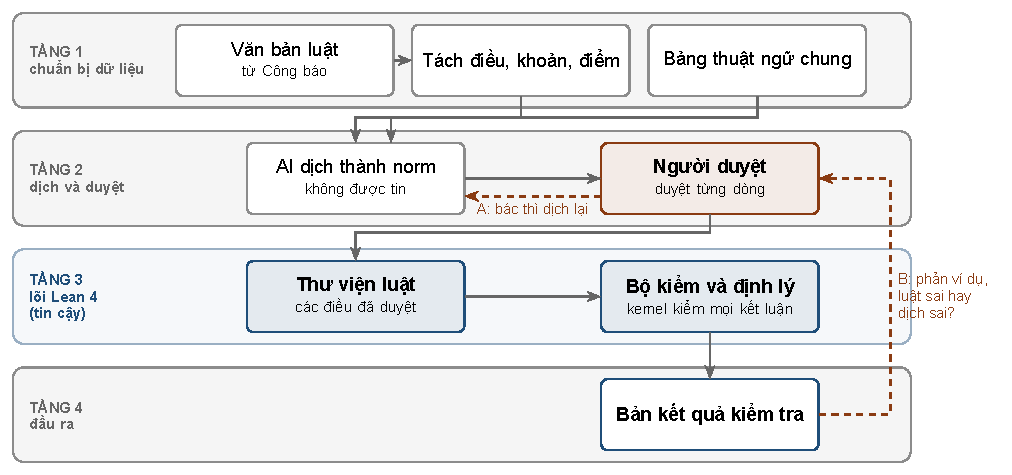
\includegraphics[width=\textwidth]{fig-hld.pdf}
\caption{Kiến trúc tổng thể (HLD) bốn tầng. Khung xanh là lõi Lean (tin cậy), khung cam là người duyệt, nét đứt cam là hai vòng
phản hồi.}
\label{fig:hld}
\end{figure}

\subsection{Các khối trong thư viện Lean}

\begin{table}[H]
\centering\small
\caption{Bốn khối của thư viện Lean.}
\begin{tabularx}{\textwidth}{>{\raggedright\arraybackslash}p{2.4cm}L}
\toprule
Khối & Nội dung\\
\midrule
\code{Core} & Kiểu dữ liệu: \code{Norm}, tính chất, điều kiện \code{Cond}, ngoại lệ, ưu tiên, nguồn; bảng atom và phép gán giá trị;
tham chiếu điều khoản có cấu trúc (\code{ClauseRef}).\\
\code{Verify} & Validator, định nghĩa \code{Conflict}, bộ kiểm theo cặp \code{analyzeP}, phần in kết quả \code{analyzeReport},
cạnh kéo theo (\code{Entail}), dấu hiệu lỗi soạn thảo (\code{Drafting}), phản ví dụ bằng lời, kiểm thử.\\
\code{Laws} & Mỗi điều đã duyệt một module (15 module), module gộp \code{Law44} và module lỗi soạn thảo
\code{Law44Drafting}.\\
\code{Cert} & Hai bước kiểm lúc build: chỉ dùng tiên đề cho phép; không module ngoài lõi gọi trực tiếp phần nội bộ của bộ
kiểm.\\
\bottomrule
\end{tabularx}
\end{table}

Phần tìm kiếm nằm trong một không gian tên nội bộ và \emph{không} được gọi trực tiếp: mọi lời gọi phải đi qua cửa vào
\code{analyzeP}, nơi validator chạy trước. Bước kiểm \code{Cert} bảo đảm quy tắc này bằng máy.

\subsection{Quy trình duyệt và truy vết}

Bảng thuật ngữ (41 hành vi, 90 atom cho Luật 44) là danh sách khái niệm dùng chung cho mọi điều: một id dùng ở hai điều là
\emph{một} khái niệm, nhờ đó hai điều luật nói về cùng một hành vi mới so được với nhau. Bảng cũng được duyệt từng mục.

Mỗi phiếu duyệt ghi sha256 của bản dịch và của bảng thuật ngữ tại thời điểm duyệt. Nếu tệp đổi sau khi duyệt, mã băm không
khớp và công cụ từ chối. Ngoại lệ duy nhất có kiểm soát: nếu bảng thuật ngữ chỉ được \emph{thêm} mục, công cụ tìm phiên bản
cũ trong lịch sử Git và chấp nhận phiếu khi mọi thuật ngữ bản dịch dùng giữ nguyên nghĩa. Module Lean sinh ra ghi lại người
duyệt, ngày duyệt, các giả định đã được chấp nhận và mã băm của mọi tệp liên quan.

\subsection{Kết quả ba giá trị và nguyên tắc «fail closed»}

Khi không chắc, hệ thống trả «không biết» thay vì đoán. Cụ thể: dữ liệu không hợp lệ (điều kiện trỏ tới atom không có,
tham chiếu không phân tích được, danh sách norm rỗng, chu trình ưu tiên) làm kết quả là \code{invalid} kèm danh sách lỗi có
tên; một điều không mã hóa phải có lý do ghi lại; mục lỗi soạn thảo không tìm được ví dụ được ghi «không biết», không bao giờ
được coi là lỗi đã chứng minh. Bản kết quả kiểm tra luôn in kèm \term{cờ rỗng}: nếu không hành vi nào mang hai tính chất trái nhau, kết
quả «nhất quán» đúng nhưng không nói gì về các điều kiện, và bản kết quả nói rõ điều đó.

\subsection{Thiết kế chi tiết lõi Lean (LLD)}

Hình~\ref{fig:lld} cho thấy luồng xử lý bên trong lõi Lean và định lý bảo đảm từng bước. Phần A là bộ kiểm xung đột: dữ liệu
của một module \code{Laws} đi qua bước kiểm dữ liệu; có lỗi thì dừng với kết quả \code{.invalid} («không biết»); không có lỗi
thì mỗi cặp norm cùng hành vi được kiểm trên các phép gán một phần; kết quả được in thành lời. Phần B là bộ kiểm lỗi soạn thảo:
chứng nhân do công cụ Python tìm được giải mã, rồi được kiểm trong Lean. Mũi tên chấm nối mỗi bước với định lý bảo đảm nó.
Chi tiết từng khai báo nằm trong \code{docs/design-core.md}.

\begin{figure}[H]
\centering
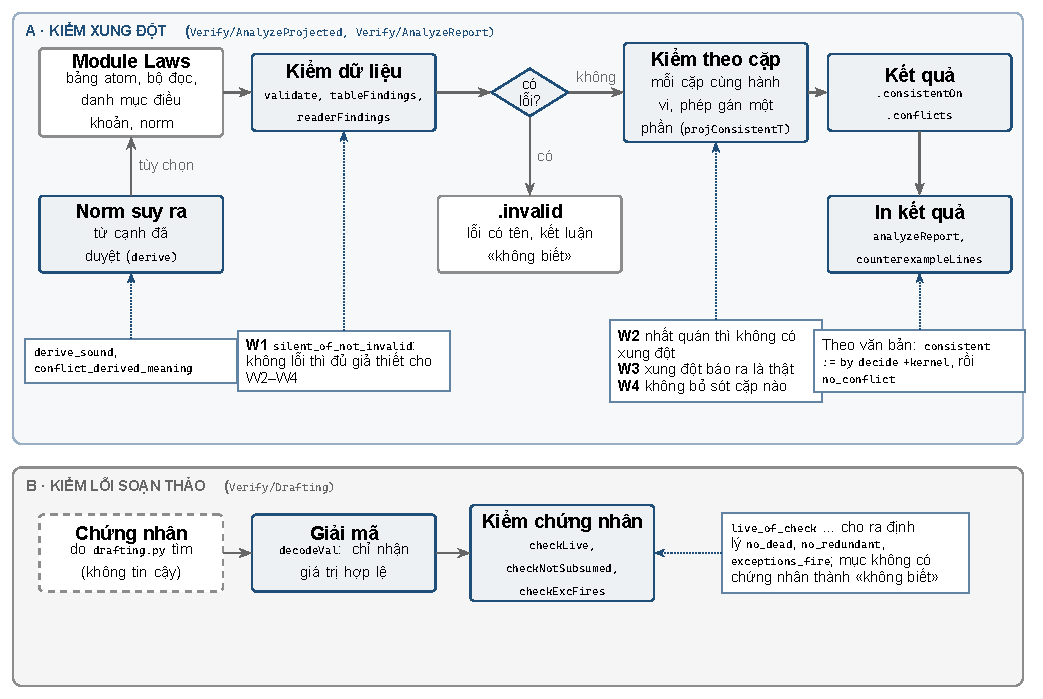
\includegraphics[width=\textwidth]{fig-lld.pdf}
\caption{Thiết kế chi tiết (LLD) của lõi Lean: bộ kiểm xung đột (A) và bộ kiểm lỗi soạn thảo (B). Khung xanh là hàm Lean;
khung viền chấm là định lý; khung nét đứt là dữ liệu không tin cậy.}
\label{fig:lld}
\end{figure}

% ================================================================ 5
\section{Mô hình dữ liệu và thuật toán}\label{sec:algo}

\subsection{Một norm trong Lean}

Điều 19 của Luật 44 liệt kê các địa điểm không được bán rượu, bia. Sau khi được duyệt, nó trở thành module Lean sau (rút
gọn):

\begin{Verbatim}
def norms : List Norm :=
  [ nrm "Điều 19:19.1" .prohibition "ban_ruou_bia" (.sit 0) [] "Điều 19 khoản 1" []
  , nrm "Điều 19:19.3" .prohibition "ban_ruou_bia"
        (.and (.sit 2) (.param 0)) [] "Điều 19 khoản 3" []
  , nrm "Điều 19:19.6" .prohibition "ban_ruou_bia" (.sit 5) [(.sit 6)]
        "Điều 19 khoản 6" [] ]
def status : ReviewStatus := .reviewed "Vũ Đức Phong" ⟨2026, 11, 24⟩
theorem silent : pfindings tS tP rS rP catalog norms = [] := by decide +kernel
\end{Verbatim}

Mỗi dòng là một norm: id mang số điều, tính chất \emph{cấm}, hành vi \code{ban\_ruou\_bia}, điều kiện (\code{.sit 0} là atom
«địa điểm là cơ sở y tế»), danh sách ngoại lệ, và nguồn. Norm 19.3 dùng một tham số (khái niệm mở «dành cho người chưa đủ 18
tuổi»); norm 19.6 có ngoại lệ «địa điểm được phép kinh doanh». Định lý \code{silent} được kernel kiểm: validator không tìm thấy
lỗi nào trong dữ liệu.

\subsection{Định nghĩa xung đột}

Một norm \emph{áp dụng} tại một tình huống khi điều kiện đúng và không ngoại lệ nào đúng. Xung đột được định nghĩa là một mệnh
đề logic, không phải một thuật toán:

\begin{Verbatim}
def Conflict (A : Atoms S P) (n₁ n₂ : Norm) (π : P) (s : S) : Prop :=
  n₁.act = n₂.act ∧                      -- cùng hành vi
  n₁.applies A π s = some true ∧          -- n₁ áp dụng tại tình huống (π, s)
  n₂.applies A π s = some true ∧          -- n₂ cũng áp dụng
  Incompatible n₁.modality n₂.modality = true ∧   -- tính chất trái nhau
  Norm.resolved n₁ n₂ = false             -- không bên nào được ưu tiên
\end{Verbatim}

Ở đây \code{s} là giá trị các atom tình huống và \code{π} là giá trị các tham số. Bộ kiểm là một hàm khác; mối liên hệ giữa
hàm kiểm và định nghĩa này được chứng minh riêng (mục~\ref{sec:link}). Cách tách này giúp người đọc chỉ cần hiểu định nghĩa
năm dòng trên để biết kết luận nói gì.

\subsection{Validator: kiểm dữ liệu trước khi tìm kiếm}

Trước khi tìm xung đột, \code{analyzeP} chạy validator và dừng nếu có bất kỳ phát hiện nào: điều kiện hoặc ngoại lệ trỏ tới
atom không tồn tại; hai norm trùng id; tham chiếu tới norm không có; danh sách norm rỗng; bảng atom có miền rỗng hoặc tên
trùng; bộ đọc trỏ tới giá trị không có; \emph{chu trình ưu tiên} (A thắng B, B thắng A, trực tiếp hoặc qua nhiều bước). Phần
phát hiện chu trình đã được chứng minh theo cả hai chiều: validator báo khi và chỉ khi có chu trình.

\subsection{Kiểm theo cặp với phép chiếu}

Cách kiểm ngây thơ là duyệt mọi tình huống: với $k$ atom đúng/sai, có $2^k$ tình huống. Bảng của Luật 44 có khoảng 87 atom,
nên $2^{87}$ là không thể. Hệ thống dùng hai nhận xét:
\begin{enumerate}
  \item Chỉ cần so các cặp norm \emph{cùng hành vi}; cặp khác hành vi không thể xung đột theo định nghĩa trên.
  \item Một norm chỉ «đọc» vài atom. Để biết hai norm có cùng áp dụng không, chỉ cần duyệt các giá trị của \emph{những atom
    mà hai norm đó đọc}; các atom còn lại có giá trị nào cũng không ảnh hưởng.
\end{enumerate}
Thuật toán: với mỗi cặp $i<j$ cùng hành vi, liệt kê mọi \emph{phép gán một phần} trên các atom mà cặp đó đọc, và kiểm xem có
phép gán nào làm cả hai áp dụng với tính chất trái nhau và không được ưu tiên giải quyết. Số điểm phải duyệt cho mỗi cặp bằng
tích kích thước miền của các atom được đọc, thường chỉ vài chục, thay vì tích trên toàn bảng.

Đo trên một cặp thật: khi thêm 1, 2, 3 atom không ai đọc vào bảng, kiểm theo cặp giữ nguyên khoảng 5 giây, còn kiểm toàn miền
tăng gấp đôi mỗi lần (5,7 → 10,7 → 21,6 → 44,2 giây). Hai cách luôn cho cùng kết quả.

\subsection{Các định lý liên kết}\label{sec:link}

Phép chiếu là một tối ưu, nên phải chứng minh nó không làm sai kết luận. Ba định lý chính:

\begin{keybox}
\begin{itemize}[leftmargin=1.2em]
  \item \textbf{Nhất quán thì không có xung đột (W2).} Nếu \code{analyzeP} trả \code{consistentOn}, thì với \emph{mọi} cặp
    norm và \emph{mọi} tình huống trên miền đầy đủ, không có \code{Conflict}. Kể cả các cặp khác hành vi bị bỏ qua.
  \item \textbf{Xung đột là thật (W3).} Nếu \code{analyzeP} trả \code{conflicts}, thì mỗi cặp được liệt kê đều có một tình
    huống cụ thể mà \code{Conflict} đúng.
  \item \textbf{Không bỏ sót (W4).} Mọi cặp cùng hành vi thực sự xung đột ở một tình huống nào đó đều được liệt kê.
\end{itemize}
\end{keybox}

Nhờ các định lý này, với mỗi văn bản chỉ cần để kernel tính \code{analyzeP} một lần. Module gộp của Luật 44 có:
\begin{Verbatim}
theorem consistent :
    analyzeP tS tP rS rP catalog norms = .consistentOn (...) := by decide +kernel
theorem no_conflict :
    ∀ n₁ ∈ norms, ∀ n₂ ∈ norms, ∀ π s, ¬ Conflict (atomsOf ...) n₁ n₂ π s
\end{Verbatim}
Định lý thứ hai được suy ra từ định lý thứ nhất và W2; nó là phát biểu mà người đọc cần: không có xung đột nào, ở đâu cả.

\subsection{Cạnh kéo theo giữa các hành vi}\label{sec:entail}

Định nghĩa \code{Conflict} chỉ so hai norm cùng hành vi. Nhưng «bắt buộc thu hồi rượu kém chất lượng» và «cấm vận chuyển rượu
kém chất lượng» là hai hành vi khác tên, trong khi thu hồi thường kéo theo vận chuyển. Để bắt loại xung đột này, hệ thống
thêm \term{cạnh} «làm A thì nhất thiết làm B» như một dữ liệu riêng, có nguồn và lời giải thích, và phải được duyệt.

Từ cạnh A ⇒ B, hệ thống \emph{suy ra} norm mới theo hai luật: cấm B kéo theo cấm A (làm A thì phải làm B, mà B bị cấm); bắt
buộc A kéo theo bắt buộc B. Quyền không được truyền. Norm suy ra giữ nguyên điều kiện, ngoại lệ và mang tiền tố «SUY RA [A ⇒
B]» trong id. Hai định lý bảo đảm ý nghĩa:
\begin{itemize}
  \item \code{derive\_sound}: ai tôn trọng các cạnh mà tuân thủ norm gốc thì cũng tuân thủ norm suy ra;
  \item \code{conflict\_derived\_meaning}: một xung đột với norm suy ra nghĩa là norm gốc áp dụng ở đó, và không cách hành động
    nào tôn trọng các cạnh lại vừa làm theo norm thứ nhất vừa tuân thủ norm gốc.
\end{itemize}

\textbf{Duyệt theo nhu cầu.} Cạnh là cách đọc, có thể sai. Thay vì bắt người duyệt xem mọi cạnh AI đề xuất, công cụ chạy Lean
với mọi cạnh chưa bị bác và chỉ đưa ra những cạnh nằm trên đường dẫn tới một cặp xung đột. Một cạnh không dẫn tới xung đột nào
thì đúng hay sai cũng không đổi kết quả; một cạnh sai mà sinh xung đột thì tự lộ ra trong danh sách phải duyệt. Kết quả có
dùng cạnh được báo ở một mục riêng và \emph{không bao giờ} đổi kết luận về chữ luật.

\subsection{Dấu hiệu lỗi soạn thảo bằng chứng nhân}

Ba tính chất được kiểm cho mọi norm của văn bản:
\begin{itemize}
  \item \code{Live}: có tình huống mà norm áp dụng (norm không chết);
  \item \code{NotSubsumed}: với hai norm cùng hành vi, cùng tính chất, có tình huống mà norm thứ nhất áp dụng còn norm thứ hai
    thì không (không bị bao trùm);
  \item \code{ExcFires}: với mỗi ngoại lệ, có tình huống mà điều kiện của norm và ngoại lệ cùng đúng (ngoại lệ có tác dụng).
\end{itemize}
Mỗi tính chất có dạng «tồn tại một tình huống». Một chương trình Python (không tin cậy) tìm cho mỗi mục một tình huống làm
\term{chứng nhân}; kernel chỉ cần \emph{kiểm} chứng nhân, việc này rẻ hơn nhiều so với tìm. Mục không tìm được chứng nhân bị
loại khỏi định lý và ghi «không biết». Hệ thống không khẳng định đó là lỗi, vì muốn khẳng định phải chứng minh một mệnh đề
«với mọi tình huống».

\subsection{Phản ví dụ bằng lời}

Khi có xung đột, Lean in tình huống gây xung đột bằng tiếng Việt: tên và nguồn hai norm, giá trị từng atom kèm khoản luật
định nghĩa nó, và ghi chú rằng mọi atom khác có thể nhận giá trị bất kỳ. Ví dụ (từ lần chạy có hai cạnh «thu hồi ⇒ vận
chuyển / tàng trữ», trước khi người duyệt bác chúng):
\begin{Verbatim}
▸ Điều 5:5.12.i.c (cấm; Điều 5 khoản 12 nhánh (i)) ×
  SUY RA [thu_hoi_xu_ly_ruou_bia ⇒ van_chuyen_ruou_bia] Điều 32:32.4 (bắt buộc)
    Tình huống:
      - ruou_bia_do_co_so_minh_san_xuat_mua_ban = đúng (nguồn: Điều 32 khoản 4)
      - ruou_bia_khong_bao_dam_chat_luong = đúng (nguồn: Điều 5 khoản 12 nhánh (i))
      - ruou_bia_gia = sai, ruou_bia_nhap_lau = sai, ...
    Mọi atom khác: giá trị bất kỳ (hai norm này không đọc chúng).
\end{Verbatim}
Phần in chỉ là trình bày; tính đúng của tình huống đã được định lý W3 bảo đảm.

% ================================================================ 6
\section{Kết quả đạt được}

\subsection{Dữ liệu và mức phủ}

\begin{table}[H]
\centering\small
\caption{Luật 44/2019/QH14 trong hệ thống (ngày 25-11-2026).}
\label{tab:coverage}
\begin{tabularx}{\textwidth}{>{\raggedright\arraybackslash}p{5.4cm}L}
\toprule
Chỉ số & Giá trị\\
\midrule
Số điều của văn bản & 36; cả 36 điều đều có trạng thái rõ ràng\\
Điều đã mã hóa và được duyệt & 15 (Điều 5, 10, 12–21, 32–34)\\
Điều ngoài phạm vi mã hóa & 21 (định nghĩa, chính sách, việc của cơ quan nhà nước, hiệu lực; người duyệt đồng ý cả 21)\\
Số norm trong module gộp & 77: 56 cấm, 16 bắt buộc, 5 cho phép\\
Bảng thuật ngữ & 41 hành vi, 90 atom; 129 mục được chấp nhận, 2 bị bác\\
Phiếu duyệt & 28 phiếu, gần 500 dòng quyết định\\
Khoản, điểm bị bỏ qua im lặng & 0: mọi đơn vị có norm hoặc lý do không mã hóa\\
\bottomrule
\end{tabularx}
\end{table}

Một số điều phải qua nhiều vòng: Điều 5 (ba lần dịch), Điều 32 và Điều 19 (hai lần), Điều 15 (ba lần). Mỗi lần bác đều có lý
do ghi trên phiếu; ví dụ ở Điều 32, người duyệt bác vì cụm «sau khi uống rượu, bia» phải áp dụng cho cả hai nhánh của khoản 6,
còn bản dịch chỉ áp dụng cho một nhánh.

\begin{table}[H]
\centering\small
\caption{Số norm theo điều trong module gộp \code{Law44}.}
\label{tab:perarticle}
\begin{tabular}{lcccc|lcccc}
\toprule
Điều & cấm & bắt buộc & cho phép & cộng & Điều & cấm & bắt buộc & cho phép & cộng\\
\midrule
5 & 19 & -- & -- & 19 & 18 & 1 & -- & -- & 1\\
10 & 6 & -- & -- & 6 & 19 & 6 & -- & -- & 6\\
12 & 9 & -- & -- & 9 & 20 & -- & 1 & -- & 1\\
13 & 2 & -- & -- & 2 & 21 & 1 & 1 & -- & 2\\
14 & 1 & -- & -- & 1 & 32 & 2 & 5 & 1 & 8\\
15 & 4 & -- & 4 & 8 & 33 & -- & 6 & -- & 6\\
16 & 4 & -- & -- & 4 & 34 & -- & 3 & -- & 3\\
17 & 1 & -- & -- & 1 & \textbf{Cộng} & \textbf{56} & \textbf{16} & \textbf{5} & \textbf{77}\\
\bottomrule
\end{tabular}
\end{table}

\subsection{Kết quả kiểm nhất quán}

\begin{keybox}
\textbf{Kết luận chính (định lý kernel \code{Law44.consistent} và \code{Law44.no\_conflict}):} trên 77 norm của 15 điều đã
duyệt, \textbf{không có xung đột} ở bất kỳ tình huống nào. Đã kiểm 165 cặp cùng hành vi; 2\,761 cặp khác hành vi được bao bởi
định lý W2.
\end{keybox}

Kết luận này cần đọc đúng mức. Trong 41 hành vi, chỉ 4 hành vi (đều ở Điều 15: cấp phép sản xuất rượu công nghiệp, cấp phép
sản xuất rượu thủ công, nhận đăng ký sản xuất rượu thủ công, cấp phép mua bán rượu) mang cả lệnh cấm và quyền. Ở 4 hành vi đó,
kết luận có nội dung: kernel chứng minh điều kiện «thiếu điều kiện thì cấm cấp phép» và «đủ điều kiện thì được cấp phép» không
bao giờ cùng đúng. Ở 37 hành vi còn lại chỉ có một tính chất, nên «nhất quán» đúng một cách hiển nhiên; bản kết quả kiểm tra nói rõ điều
này. Luật 44 chủ yếu gồm lệnh cấm và nghĩa vụ, nên xung đột theo nghĩa hẹp (cùng hành vi) hiếm là điều có thể dự đoán.

Hai định lý \code{covers\_articles} và \code{covers\_articles\_source} chứng minh danh sách norm của module gộp đúng bằng norm
của 15 module từng điều (id, tính chất, hành vi, nguồn, tham chiếu, số ngoại lệ), nên việc gộp không làm mất hay thêm norm.

Bảng~\ref{tab:law44thm} liệt kê mọi định lý Lean mà kết quả trên Luật 44 dựa vào. Tất cả được kernel kiểm lại mỗi lần build.

\begin{table}[H]
\centering\small
\caption{Các định lý Lean trên Luật 44/2019/QH14 và điều chúng bảo đảm.}
\label{tab:law44thm}
\begin{tabularx}{\textwidth}{>{\raggedright\arraybackslash}p{5.6cm}L}
\toprule
Định lý (module) & Bảo đảm\\
\midrule
\code{refs\_parse} (\code{Law44}) & Mọi tham chiếu điều khoản trong module đều phân tích được\\
\code{silent} (\code{Law44}) & Validator, kiểm bảng atom và kiểm bộ đọc không tìm thấy lỗi nào\\
\code{consistent} (\code{Law44}) & Bộ kiểm trả «nhất quán trên phần đã mã hóa» (kernel tự tính)\\
\code{no\_conflict} (\code{Law44}) & Không có cặp norm nào xung đột ở bất kỳ tình huống nào\\
\code{covers\_articles}, \code{covers\_articles\_source} & Module gộp đúng bằng 15 module từng điều\\
\code{no\_dead} (\code{Law44Drafting}) & 77/77 norm có tình huống áp dụng\\
\code{no\_redundant} (\code{Law44Drafting}) & 322 cặp cùng hành vi, cùng tính chất: không norm nào bị bao trùm\\
\code{exceptions\_fire} (\code{Law44Drafting}) & 6/6 ngoại lệ có tình huống kích hoạt\\
\bottomrule
\end{tabularx}
\end{table}

\subsection{Thử nghiệm gieo lỗi}

Để biết bộ kiểm có bắt được xung đột khi xung đột tồn tại, các xung đột được gieo nhân tạo vào bản mã hóa thật:
\begin{itemize}
  \item \textbf{Đổi tính chất trên cùng hành vi} (ví dụ thêm một bản sao «cho phép» của một lệnh cấm): bắt \textbf{23/23}.
  \item \textbf{Đối chứng âm}: bản sao có điều kiện phủ định, nên hai norm không bao giờ cùng áp dụng: \textbf{0/23} báo
    nhầm.
  \item \textbf{Hành vi khác tên}: trong 12 ca đổi sang một hành vi gần nghĩa, chỉ 3 ca là xung đột thật theo định nghĩa «tuân
    thủ kéo theo vi phạm». Không có cạnh thì bắt 0/3; có cạnh kéo theo thì bắt 3/3, và không báo nhầm ca nào trong 9 ca còn
    lại.
\end{itemize}
Thử nghiệm cuối chỉ cho thấy Lean thực hiện đúng ngữ nghĩa của cạnh, vì nhãn «nên bắt» được tính từ chính các cạnh; cần đọc
kết quả này với giới hạn đó.

\subsection{Nghiên cứu trường hợp 1: Điều 32 khoản 4 và Điều 5 khoản 12}

AI đề xuất 13 cạnh kéo theo. Cơ chế duyệt theo nhu cầu chỉ ra rằng chỉ \textbf{2/13} cạnh nằm trên đường dẫn tới xung đột:
«thu hồi ⇒ vận chuyển» và «thu hồi ⇒ tàng trữ». Với hai cạnh này, kernel chứng minh có xung đột (43 giây) giữa:
\begin{itemize}
  \item Điều 32 khoản 4: cơ sở kinh doanh \emph{phải} thu hồi rượu, bia không bảo đảm chất lượng do mình sản xuất, mua bán;
  \item Điều 5 khoản 12: \emph{cấm} kinh doanh, tàng trữ, vận chuyển rượu, bia không bảo đảm chất lượng.
\end{itemize}
Một cạnh thử nghiệm cố ý sai được thêm vào làm đối chứng; nó tự lộ ra với 16 cặp xung đột vô lý, đúng như thiết kế.

Hệ thống chạy thêm ba cách đọc: R0 (theo đúng chữ: có xung đột), R1 (lệnh cấm chỉ nhắm việc kinh doanh: nhất quán), R2
(thu hồi là ngoại lệ ngầm theo nguyên tắc quy định riêng thắng quy định chung: nhất quán). Người duyệt quyết: \textbf{bác cả
hai cạnh} (rượu chưa bán ra có thể xử lý tại chỗ, không cần vận chuyển; «tàng trữ» là giữ để bán, không phải nghĩa của «thu hồi
và xử lý») và chọn R2 cho hồ sơ. Ứng viên xung đột vì vậy bị loại. Trường hợp này minh họa trọn vòng: máy phát hiện, máy thu
hẹp việc phải duyệt (2 thay vì 13 cạnh), con người quyết, và quyết định được ghi lại có kiểm được.

\subsection{Nghiên cứu trường hợp 2: ngoại lệ không có tác dụng ở Điều 15}

Lần kiểm lỗi soạn thảo đầu tiên trên 73 norm cho kết quả: 73/73 norm sống, 322 cặp không bao trùm, 5/6 ngoại lệ có tác dụng,
và \textbf{1 mục «không biết»}: ngoại lệ «trừ trường hợp quy định tại khoản 3» của Điều 15 khoản 2 không bao giờ kích hoạt.
Nguyên nhân: bản mã hóa cũ đặt danh sách chủ thể của khoản 2 (doanh nghiệp, hợp tác xã, hộ kinh doanh) vào \emph{phạm vi} của
norm, trong khi luật ghi nó là \emph{một điều kiện cấp phép} (điểm a). Khi phạm vi đã loại hộ gia đình, ngoại lệ dành cho hộ
gia đình không còn chỗ để có tác dụng.

Câu hỏi được chuyển cho người duyệt; Điều 15 được dịch lại hai lần nữa theo các câu trả lời (thêm chiều «đủ điều kiện thì được
cấp phép»; coi việc đăng ký với UBND cấp xã ở khoản 3 là tương đương cấp phép). Sau lần 3, được duyệt 24/24 dòng:

\begin{table}[H]
\centering\small
\caption{Trước và sau khi dịch lại Điều 15.}
\begin{tabular}{lcc}
\toprule
 & Trước & Sau\\
\midrule
Số norm & 73 & 77\\
Ngoại lệ có tác dụng & 5/6 & \textbf{6/6}\\
Mục «không biết» & 1 & \textbf{0}\\
Hành vi có cả cấm và cho phép & 0 (kết luận rỗng) & \textbf{4}\\
\bottomrule
\end{tabular}
\end{table}

Đây là một ví dụ về giá trị của việc kiểm lỗi soạn thảo: tín hiệu không phải là lỗi của luật, mà là lỗi của \emph{bản mã hóa},
và nó được phát hiện mà không cần ai đọc lại cả điều.

\subsection{Hiệu năng và quy mô mã}

\begin{table}[H]
\centering\small
\caption{Thời gian kernel và quy mô (máy tính xách tay, Windows 11).}
\begin{tabularx}{\textwidth}{>{\raggedright\arraybackslash}p{7.4cm}L}
\toprule
Hạng mục & Số đo\\
\midrule
Build \code{Law44} (77 norm, gồm \code{consistent} và \code{covers\_*}) & khoảng 5,5 phút\\
Kernel kiểm \code{Law44Drafting} (77 norm, 322 cặp, 6 ngoại lệ) & khoảng 80 giây\\
Kernel chứng minh xung đột với hai cạnh thu hồi & 43 giây\\
Mã Lean & khoảng 13\,000 dòng, hơn 300 định lý\\
Mã Python (công cụ) & khoảng 6\,800 dòng, 150 kiểm thử tự động\\
Lịch sử & 113 commit (từ 20-10-2026), 31 bản ghi quyết định thiết kế\\
\bottomrule
\end{tabularx}
\end{table}

Toàn bộ quy trình có thể chạy lại bằng một lệnh (\code{python pipeline/demo.py}): build, sinh bản kết quả kiểm tra, gieo một xung đột để
thấy hệ thống bắt nó, chạy cạnh kéo theo, các cách đọc và kiểm lỗi soạn thảo; mọi đầu ra ghi vào một thư mục riêng.

% ================================================================ 7
\section{Vấn đề gặp phải và cách giải quyết}

Bảng~\ref{tab:problems} tóm tắt các vấn đề chính gặp trong quá trình làm, theo thứ tự từ đầu vào tới bản kết quả kiểm tra. Mỗi cách giải
quyết đều có bản ghi quyết định (ADR) hoặc ghi chép trong \code{docs/} và \code{eval/}.

\begin{longtable}{>{\raggedright\arraybackslash}p{4.1cm}>{\raggedright\arraybackslash}p{6.0cm}>{\raggedright\arraybackslash}p{4.3cm}}
\caption{Vấn đề, cách giải quyết và kết quả đo được.}\label{tab:problems}\\
\toprule
Vấn đề & Cách giải quyết & Kết quả\\
\midrule
\endfirsthead
\toprule
Vấn đề & Cách giải quyết & Kết quả\\
\midrule
\endhead
\bottomrule
\endfoot
LLM dịch sai nghĩa, bịa trích dẫn hoặc bỏ sót phạm vi &
Công cụ kiểm: trích dẫn phải nằm nguyên văn trong khoản được dẫn, id phải có trong bảng thuật ngữ. Người duyệt từng norm và
từng giả định; bác một giả định thì phải dịch lại. &
28 phiếu, gần 500 dòng quyết định; Điều 5 và Điều 15 dịch 3 lần, Điều 19 và Điều 32 dịch 2 lần.\\
Các điều không so được với nhau vì mỗi bản dịch đặt tên atom và hành vi riêng &
Bảng thuật ngữ dùng chung cho cả văn bản: một id là một khái niệm; mỗi mục được duyệt (ADR-0027). &
41 hành vi, 90 atom; 129 mục chấp nhận, 2 bác; 5 phiếu bảng thuật ngữ.\\
Bùng nổ tổ hợp: khoảng 87 atom, $2^{87}$ tình huống &
Chỉ so cặp cùng hành vi; mỗi cặp chỉ duyệt các atom hai norm đọc (phép chiếu); chứng minh W2--W4 rằng kết luận không đổi. &
Kiểm theo cặp giữ khoảng 5 giây khi thêm 3 atom; toàn miền tăng tới 44,2 giây. 165 cặp cho 77 norm.\\
Kết luận «nhất quán» rỗng: không hành vi nào mang hai tính chất trái nhau &
In cờ rỗng trong mọi bản kết quả kiểm tra; thêm cạnh kéo theo (ADR-0029) và kiểm lỗi soạn thảo (ADR-0030) để có kiểm có nội dung. &
Sau khi dịch lại Điều 15: 4 hành vi có cả cấm lẫn cho phép, kết luận có nội dung ở đó.\\
AI đề xuất nhiều cạnh, người duyệt không xem hết được &
Duyệt theo nhu cầu: chạy Lean với mọi cạnh chưa bị bác, chỉ đưa ra cạnh nằm trên đường tới xung đột. &
2/13 cạnh phải duyệt; một cạnh cố ý sai tự lộ ra với 16 cặp xung đột vô lý.\\
Phiếu đã duyệt mất hiệu lực khi bảng thuật ngữ chỉ được thêm mục (sha256 đổi) &
Tìm phiên bản bảng mang sha256 cũ trong lịch sử Git; phiếu dùng tiếp nếu mọi thuật ngữ bản dịch dùng giữ nguyên nghĩa. &
Thêm 1 hành vi cho Điều 15 mà 14 phiếu của các điều khác không phải duyệt lại.\\
Dấu hiệu lỗi soạn thảo: một ngoại lệ không bao giờ kích hoạt (Điều 15 khoản 2) &
Ghi «không biết», hỏi người duyệt; nguyên nhân là bản mã hóa đặt danh sách chủ thể vào phạm vi thay vì điều kiện; dịch lại. &
6/6 ngoại lệ có tác dụng, 0 «không biết».\\
Kernel quá thời gian khi chứng nhân viết dưới dạng giá trị Lean có kèm chứng minh &
Chứng nhân là danh sách số thô; một bộ giải mã (\code{decodeVal}) chỉ nhận giá trị hợp lệ, kernel kiểm trên đó. &
77 norm, 322 cặp, 6 ngoại lệ được kiểm trong khoảng 80 giây.\\
\code{decide} không tìm được thủ tục quyết định cho phép so bộ 6 trường &
Tách định lý so module gộp với module từng điều thành hai định lý, mỗi định lý 3 trường. &
\code{covers\_articles} và \code{covers\_articles\_source} được kernel chấp nhận.\\
Promote lại Điều 15 bị chặn vì module gộp cũ làm build thất bại &
Gỡ tạm module gộp, promote theo thứ tự: module điều, module gộp, module lỗi soạn thảo. Promote tự hoàn tác khi build lỗi. &
Build đủ 90 job đạt, kể cả hai bước kiểm tiên đề và encapsulation.\\
Đếm sai trong thử nghiệm: lần đầu báo «12/12 ca hành vi gần nghĩa bị lọt» &
Đo lại theo định nghĩa «tuân thủ kéo theo vi phạm»; ghi đính chính trong \code{eval/entailment/README.md}. &
Chỉ 3/12 là xung đột thật; bắt 3/3 khi có cạnh, 0/9 báo nhầm.\\
Không có ngân sách gọi API của LLM &
Dịch dán tay theo câu lệnh mẫu, lưu câu lệnh và kết quả (\code{eval/translate/RECORD.md}). &
Không tốn chi phí API; câu lệnh và bản dịch của mọi lần đều được lưu lại.\\
Bản kết quả kiểm tra có thể bị sửa tay hoặc đọc quá mức &
Bản kết quả chỉ do \code{report.py} sinh; từ chối trạng thái «đã duyệt» khi chưa có ca của chuyên gia; luôn in phạm vi và «Không
phải tư vấn pháp lý». &
Bản kết quả \code{law44} ở trạng thái bản nháp, có đủ 9 mục.\\
\end{longtable}

\section{Giới hạn}

\begin{warnbox}
Các giới hạn dưới đây được ghi trong chính bản kết quả kiểm tra do hệ thống sinh ra; chúng không làm sai kết quả hình thức, nhưng giới hạn
những gì kết quả đó nói về luật.
\end{warnbox}

\begin{itemize}
  \item \textbf{Một người duyệt.} Mọi bản mã hóa do một người (sinh viên, không phải chuyên gia pháp lý) duyệt. Chưa có bộ ca
    kiểm thử do người học luật trả lời độc lập, nên hệ thống từ chối sinh bản kết quả ở trạng thái «đã duyệt» và chỉ sinh «bản nháp».
  \item \textbf{Kết luận chỉ có nội dung ở Điều 15.} Ở 37 hành vi chỉ mang một tính chất, «nhất quán» là hiển nhiên.
  \item \textbf{Atom độc lập.} Các atom được coi là độc lập. Ví dụ «hộ kinh doanh» và «hộ gia đình, cá nhân» là hai atom riêng;
    theo người duyệt hai nhóm tách nhau, nhưng ràng buộc đó chưa được mã hóa, nên Lean xét cả tình huống không thể xảy ra. Điều
    này không làm sai kết luận «nhất quán» (không xung đột ở mọi tình huống thì càng không ở tình huống thật), nhưng có thể sinh
    xung đột không có thật nếu sau này có.
  \item \textbf{Cạnh và cách đọc là dữ liệu được tin.} 11 cạnh AI đề xuất chưa được duyệt (không nằm trên đường xung đột nào).
    Cạnh còn thiếu có thể che xung đột thật; chỉ người đọc luật đề xuất thêm mới bù được.
  \item \textbf{Phạm vi mã hóa.} 21 điều không được mã hóa theo một quy ước phân loại (ví dụ nghĩa vụ của cơ quan nhà nước không
    được mã hóa); đó là lựa chọn phạm vi, không phải nhận định rằng các điều đó không có chuẩn mực.
  \item \textbf{Level 2 chưa làm.} Văn bản hướng dẫn (nghị định) có thể thêm điều kiện; ví dụ chiều «đủ điều kiện thì được cấp
    phép» ở Điều 15 có thể quá rộng khi xét cả nghị định.
  \item \textbf{Dịch dán tay.} Bước dịch dùng LLM theo cách dán tay, chưa tự động hóa; thời gian build tăng theo số norm.
\end{itemize}

% ================================================================ 8
\section{Kết luận và hướng phát triển}

Dự án đã xây dựng một hệ thống hoàn chỉnh từ văn bản luật tiếng Việt tới bản kết quả kiểm tra có chứng minh: tách văn bản, dịch bằng AI,
duyệt bằng người có truy vết, đưa vào thư viện Lean, kiểm xung đột với các định lý bảo đảm ý nghĩa của kết quả, mở rộng sang
xung đột giữa các hành vi khác tên và dấu hiệu lỗi soạn thảo, và sinh bản kết quả kiểm tra bằng tiếng Việt, có phản ví dụ bằng lời. Trên Luật
44/2019/QH14, kernel chứng minh 77 norm của 15 điều không có xung đột; hai «tín hiệu» mà hệ thống đưa ra đều được con người xem
xét và giải quyết, một tín hiệu dẫn tới sửa bản mã hóa.

Lean 4 là trục của toàn bộ hệ thống: nó định nghĩa thế nào là xung đột, chạy bộ kiểm, chứng minh một lần cho mọi văn bản rằng bộ
kiểm đúng, để kernel kiểm từng kết luận cụ thể, giữ thư viện luật đã duyệt và chặn mọi chứng minh dở dang ngay lúc build. Nhờ đó,
315 định lý và một kernel nhỏ thay cho việc phải tin hàng nghìn dòng mã Python và đầu ra của một mô hình ngôn ngữ.

Điều quan trọng hơn con số là \emph{cách làm}: tách bạch cái máy chứng minh được (tính đúng hình thức) với cái chỉ con người
xác nhận được (tính trung thực với luật), không bao giờ kết luận vượt quá phần đã mã hóa, và trả «không biết» thay vì đoán.

Hướng phát triển:
\begin{enumerate}
  \item Bộ ca kiểm thử do người học luật trả lời độc lập, và người duyệt thứ hai, để đo độ trung thực.
  \item Ràng buộc giữa các atom (ví dụ hai nhóm chủ thể tách nhau) để loại tình huống không thể xảy ra.
  \item Thử trên một văn bản có nhiều quyền hơn (nơi xung đột cấm và cho phép dễ xuất hiện).
  \item Level 2: nhiều văn bản, thứ bậc hiệu lực, thời điểm có hiệu lực.
  \item Viết thành bài báo khoa học (mục tiêu: tạp chí \emph{Artificial Intelligence and Law}).
\end{enumerate}

% ================================================================ Tham khảo
\begin{thebibliography}{99}\small
\bibitem{kelsen} H. Kelsen. \emph{General Theory of Norms}. Oxford University Press, 1991.
\bibitem{vranes} E. Vranes. The Definition of `Norm Conflict' in International Law and Legal Theory. \emph{European Journal of
International Law} 17(2), 2006.
\bibitem{catala} D. Merigoux, N. Chataing, J. Protzenko. Catala: A Programming Language for the Law. \emph{ICFP}, 2021.
arXiv:2103.03198.
\bibitem{ncheck} N. Feng và cs. Analyzing and Debugging Normative Requirements via Satisfiability Checking. \emph{ICSE},
2024. arXiv:2401.05673.
\bibitem{robaldo} L. Robaldo, G. L. Pozzato. Conflict-tolerant Deontic Traditional Scheme. 2024. arXiv:2411.19918.
\bibitem{tnorm} N. Fornara và cs. T-NORM: modelling norms and their operational semantics. 2021.
\bibitem{horner} Horner, Mateis, Governatori, Ciabattoni. Toward Robust Legal Text Formalization into Defeasible Deontic Logic
using LLMs. 2025. arXiv:2506.08899.
\bibitem{irc} Yadamsuren, Platt, Diaz. LLM-Assisted Formalization Enables Deterministic Detection of Statutory Inconsistency
in the Internal Revenue Code. 2025. arXiv:2511.11954.
\bibitem{lean} L. de Moura, S. Ullrich. The Lean 4 Theorem Prover and Programming Language. \emph{CADE-28}, 2021.
\bibitem{luat44} Quốc hội. Luật Phòng, chống tác hại của rượu, bia số 44/2019/QH14. Công báo số 559 + 560, 17-7-2019.
\end{thebibliography}

% ================================================================ Phụ lục
\appendix
\section{Hướng dẫn chạy}

\begin{Verbatim}
# kernel kiểm mọi định lý và hai bước kiểm (khoảng 6 phút)
lake build
# chạy toàn bộ quy trình minh họa
python pipeline/demo.py --no-build
# sinh bản kết quả kiểm tra vào reports/
python pipeline/report.py --module law44 --status draft
# kiểm thử Python
python -m unittest discover -s pipeline/tests
\end{Verbatim}

Mã nguồn, tài liệu thiết kế (\code{docs/}), các phiếu duyệt đã điền (\code{docs/review/}) và bản kết quả kiểm tra do hệ thống sinh ra
(\code{reports/law44-2026-11-25.md}) đều nằm trong kho mã của dự án.

\end{document}
